
Q-learning base algorithm shows the iterative update rule for an action value function, which is said to find optimality for any FMDP assuming infinite exploration.


$Q^{n e w}\left(s_{t}, a_{t}\right) \leftarrow(1-\alpha) \cdot \underbrace{Q\left(s_{t}, a_{t}\right)}_{\text {old value }}+\underbrace{\alpha}_{\text {learning rate }} \cdot \overbrace{(\underbrace{r_{t}}_{\text {reward }} +  \underbrace{\gamma}_{\text {discount factor }}\cdot \underbrace{\max_{a}Q\left(s_{t+1}, a\right))}_{\text{estimate of optimal future value}}}^{\text {learned value }}$

\noindent
With learning rate $\alpha$, reward $r_t$ for moving into $s_{t+1}$ from $s_t$ taking action $a$ and the discount factor $\gamma$, which controls how important the future rewards are, or how much into the future the model looks.\\

\noindent
On top of the basic algorithm, DQN is a functional approximation variant of the Q-learning, in which the model is supposed to be deep (more than one layer). We used a delayed network (updated every 20 episodes) to compute the delayed values and tried both GLIE epsilone-greedy as well as a linear decaying $\epsilon$ of the form of $\frac{5mil-SF}{5mil}$, with $SF$ being the total number of frames out of all episodes seen so far, and capped it's minimum epsilon value to $\epsilon=0.1$. We noticed that having the model around episode 50k with about $50\%$ win-rate and $\epsilon=0.1$ actually worsened the model from that point onwards, so we capped $\epsilon$ to 0.3 untill episode 125000 and have it linearly decrease until 160000 (where it reached 0.1).\\

\noindent
Figure 2 shows the two main data augmentation/preprocessing we ended up doing for the dqn models. Aside from down and gray-scaling presented in the "Processing Pipeline" section, we vertically stacked 3 images (current state-image and 2 more from the 2 previous time steps). We also tried stacking them on a 3rd dimension, like the channels of an RGB image and have according convolution layers, but it seemed a little bit worse than putting the images on top of each other. For the first two time steps, where only one or two images have been seen in the episode respectively, we duplicated the first image 3 or 2 times and trained with the same input dimension (of $150\times 50$)\\



\begin{figure}[!htb]
    \centering
    \begin{subfigure}{.49\textwidth}
        \centering
        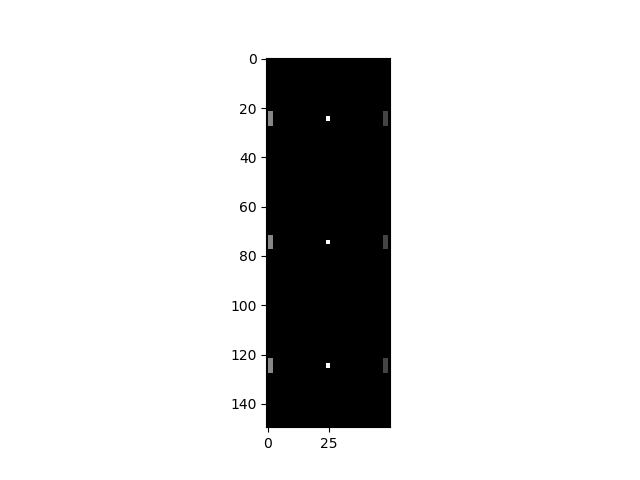
\includegraphics[width=\textwidth]{figures/dqn_training_image.png}
        \caption{Preprocessed 3-stacked images}
        \label{fig-raw}
    \end{subfigure}
    \begin{subfigure}{0.49\textwidth}
        \centering
        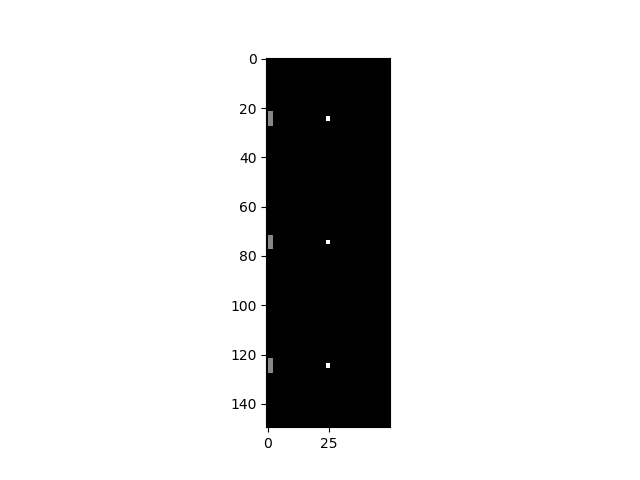
\includegraphics[width=\textwidth]{figures/dqn_training_image_blacked_out_pallet.png}
        \caption{Preprocessed 3-stacked images with blacked-out pallet}
        \label{fig-bw}
    \end{subfigure}
    \caption{DQN image augmentation and processing}
    \label{fig-small}
    \label{fig-process}
\end{figure}

\noindent
The image stacking itself is necessary due to the intrinsic issue that the process has: given only the current image as state-input to the model, it is not possible to tell the speed and direction of the ball. Therefore, the process is not Markovian, and this problem can be mitigated using past states (images) along with the current one in the training.

\noindent
The idea behind leaving the right pallet blacked out, came after we noticed that the model was doing decently against simple-ai (around $60\%$ win-rate), while having around $50\%$ against Karpathy. Rendering it, we noticed that that the dqn model probably learned that it's highes action-values, are those that get it's pole into the same position as the simple-ai model (it was imitating it), and the 60\% (so "better" than simple-ai) was probably a mere consequence of the delay with which it went to catch the ball, catching it with the edge, speeding it up and winning a little bit more often.\\ \\

\noindent
The model architecture that ended up being good enough to beat simple-ai on 80\%+, was composed of two convolution layers, with max-pooling layers in between, followed by two linear layers, $9792x120$ and $120x3$:

    \begin{minted}{python}
            Conv2d(channels, 32, kernel_size=(7, 7), stride=1)
            MaxPool2d(kernel_size=(2, 2))
            Conv2d(32, 32, kernel_size=(5, 5), stride=1)
            MaxPool2d(kernel_size=(2, 2))
		Linear(9792, 120)
		Linear(120, 3)
	\end{minted}
	
\noindent
Due to the reward sparsity, we decided to give small rewards for every non-final time step (e.g. $r=0.01$). This lead to the model learning to just "stay alive" in the first tens of thousands of iterations, but it helped quite a lot with learning in the early stages, where it is very hard to learn how to win (against simple-ai, it was clearly not enough for the model to learn to catch the ball in order to win). Usually it has to hit it with it's edge, in order to give speed and angle to the ball, for simple-ai to not be able to catch it by just following it anymore. We concluded that this should be way too difficult to learn from the start, and learning to at least catch the ball, might have more chances to produce more wins.

\noindent
We used experience replay with a buffer size of 250000 and a batch size of 32 during training, with the images stacked as described above and shown in Figure 2.

\medskip
\noindent
DQN seems like a natural choice for the problem at hand. The action space being so small (only 3 possible actions) suggests that Q value function is feasible to learn and the non-markovian property of the process (dependent on past states, given that the states represent only pixels at the current time step of each episode) is easily dealt with memory augmentation. In what follows in the results and conclusion section, we will see that the simple (almost) vanilla DQN is definitely not trivial to learn, having to account for factors like the amount of exploration, model architecture, the way the images are augmented, training parameters like replay-buffer size (which can't be too large because of memory issues), batch size and so on.
